\documentclass[11pt,a4paper]{article}
\usepackage[utf8]{inputenc}
\usepackage[spanish,es-noquoting]{babel}
\usepackage{amsmath,amsfonts,amssymb}
\usepackage{geometry}
\geometry{top=2.5cm, bottom=2.5cm, left=2.5cm, right=2.5cm}
\usepackage{hyperref}
\usepackage{booktabs}
\usepackage{tabularx}
\usepackage{xcolor}
\usepackage{tcolorbox}
\usepackage{enumitem}
\usepackage{graphicx}

% Colores institucionales
\definecolor{primary}{RGB}{15, 32, 67}
\definecolor{secondary}{RGB}{0, 114, 206}
\definecolor{lightgray}{RGB}{245, 247, 250}

\hypersetup{
    colorlinks=true,
    linkcolor=secondary,
    urlcolor=secondary,
    pdftitle={Portafolio de Evidencias No. 3 - StatCredit AI}
}

\begin{document}

% ---------------------------------------------------------
% PORTADA INSTITUCIONAL
% ---------------------------------------------------------
\begin{titlepage}
    \centering
    \vspace*{1cm}
    {\Huge \textbf{UNIVERSIDAD EXTERNADO DE COLOMBIA}}\\[0.4cm]
    {\Large \textbf{PREGRADO EN CIENCIA DE DATOS --- EMPRENDIMIENTO}}\\[1.8cm]
    
    \rule{\linewidth}{0.8mm}\\[0.4cm]
    {\Huge \textbf{PORTAFOLIO DE EVIDENCIAS NO. 3}}\\[0.3cm]
    {\Large \textbf{Validaci\'on de Campo, Segmento de Clientes y Prototipo de Valor}}\\[0.4cm]
    \rule{\linewidth}{0.8mm}\\[1.8cm]
    
    \begin{tcolorbox}[colback=primary!5,colframe=primary]
        \centering \Huge
        \textbf{StatCredit AI}
    \end{tcolorbox}
    
    \vfill
    
    \begin{minipage}{0.8\textwidth}
        \centering
        \textbf{\large Integrantes (Grupo 5):}\\[0.3cm]
        Santiago Sandoval \quad $\vert$ \quad Sebasti\'an Ramos\\[0.15cm]
        Juli\'an Duarte \quad $\vert$ \quad Tom\'as Rinc\'on \quad $\vert$ \quad Juli\'an Jim\'enez
    \end{minipage}
    
    \vfill
    {\large \textbf{Octubre de 2026 --- Bogot\'a D.C., Colombia}}
\end{titlepage}

\newpage
\tableofcontents
\newpage

% ---------------------------------------------------------
% SECCIÓN 1: VALIDACIÓN CUALITATIVA CON EXPERTOS
% ---------------------------------------------------------
\section{Evidencias de Campo: Entrevistas con Expertos del Sector}

\begin{tcolorbox}[colback=primary!5,colframe=primary,title={\textbf{\textquestiondown De qu\'e trata este entregable?}}]
En esta secci\'on presentamos los resultados de las entrevistas en profundidad que realizamos a dos expertos del sector financiero en Colombia: un ejecutivo con a\~nos de experiencia evaluando cr\'editos de consumo y una analista experta en normas de riesgo SARC de la Superintendencia Financiera. El prop\'osito fue validar directamente en el terreno si la falta de herramientas para leer extractos digitales y el temor a las auditor\'ias representan dolores reales en las entidades financieras.
\end{tcolorbox}

\subsection{Los Expertos que Entrevistamos}
\begin{itemize}[leftmargin=*]
    \item \textbf{Diego Ramos (Experto en Riesgo Crediticio):} Profesional con amplia trayectoria en comit\'es de cr\'edito y evaluaci\'on de consumo. Conoce de primera mano c\'omo operan los analistas y por qu\'e se descarta a solicitantes independientes que s\'i tienen solvencia.
    \item \textbf{Paola C\'ardenas (Analista Microempresarial y Experta SARC):} Especialista en regulaci\'on financiera y cumplimiento del Sistema de Administraci\'on del Riesgo Crediticio (SARC) ante la Superintendencia Financiera de Colombia.
\end{itemize}

\subsection{Transcripci\'on de las Entrevistas}

\subsubsection{Entrevista 1: Diego Ramos (Riesgo Crediticio)}

\begin{tcolorbox}[colback=lightgray,colframe=primary,title={\textbf{Pregunta 1: Rechazo de independientes por falta de historial en bur\'o}}]
\textit{\textquestiondown Ustedes rechazan mucha gente independiente por lo del tema de DataCr\'edito y esas cosas?}
\tcblower
\textbf{Respuesta de Diego Ramos:}  
«S\'i, much\'isimo, m\'as de lo que se cree normalmente. Yo llevaba a\~nos en eso y apenas el sistema ve que el cliente no tiene un puntaje bueno en el bur\'o, ni siquiera llega a que un analista lo mire con calma. Y muchas veces ese se\~nor s\'i tiene con qu\'e pagar por lo que puede decirnos m\'as personalmente, solo que nunca tuvo una tarjeta de cr\'edito o nunca sac\'o un pr\'estamo formal, entonces para el sistema es como si no existiera.»
\end{tcolorbox}

\begin{tcolorbox}[colback=lightgray,colframe=primary,title={\textbf{Pregunta 2: Capacidad de revisar extractos a mano}}]
\textit{\textquestiondown Y si la persona le muestra los movimientos de Nequi o las facturas, ustedes tienen c\'omo revisar eso r\'apido?}
\tcblower
\textbf{Respuesta de Diego Ramos:}  
«No, y ah\'i es donde hay un problema ya que eso tocar\'ia revisarlo a mano, uno abriendo el PDF del extracto, contando transacci\'on por transacci\'on, sacando el promedio en Excel y as\'i uno alcanza a sacar m\'aximo 15 o 20 casos al d\'ia por persona. Pero no es que no queramos usar esa informaci\'on, es que no damos abasto para procesarla cuando hay tantas personas que manejan el dinero de esa manera. Si a m\'i me hubieran dado algo autom\'atico que me diera bien la informaci\'on como lo que me cuentas que quieren hacer, eso me cambiar\'ia la manera de c\'omo se rechazar\'ia a los clientes.»
\end{tcolorbox}

\begin{tcolorbox}[colback=lightgray,colframe=primary,title={\textbf{Pregunta 3: Comportamiento de pago de independientes vs. asalariados}}]
\textit{\textquestiondown Un independiente que mueve plata todos los d\'ias es m\'as moroso que uno con sueldo fijo?}
\tcblower
\textbf{Respuesta de Diego Ramos:}  
«No, y digamos que eso lo sabemos todos los que trabajan en esto, aunque no se mencione mucho. Yo he visto casos de gente que tiene su negocio como yo y le entra plata todos los d\'ias, y hay m\'as organizados que muchos asalariados que conozco. Lo que pasa es que a uno en el banco lo criaron con el cuento de que `n\'omina fija es igual a seguridad', y es como que ese chip es dif\'icil de cambiar para que la gente de un d\'ia para otro revise otras perspectivas.»
\end{tcolorbox}

\begin{tcolorbox}[colback=lightgray,colframe=primary,title={\textbf{Pregunta 4: Miedo a aprobar cr\'editos sin certificado laboral}}]
\textit{\textquestiondown Y qu\'e tanto miedo le tienen ustedes a aprobar un cr\'edito sin el desprendible de n\'omina de toda la vida?}
\tcblower
\textbf{Respuesta de Diego Ramos:}  
«El miedo no es nuestro sino del banco, porque muchas personas nos cuentan sus historias y de manera hablada catalogan para poder entrar a revisi\'on pero sin las herramientas deja de ser posible. Si yo apruebo algo raro y despu\'es algo sale mal, quien tiene que ir a dar la cara en el comit\'e de auditor\'ia soy yo. Entonces pues uno prefiere por si las moscas, decir que no de una vez, as\'i uno sepa que se le est\'a negando el pr\'estamo a alguien que seguramente s\'i paga.»
\end{tcolorbox}

\subsubsection{Entrevista 2: Paola C\'ardenas (Regulaci\'on SARC)}

\begin{tcolorbox}[colback=lightgray,colframe=secondary,title={\textbf{Pregunta 1: Exigencias de la Superfinanciera sobre algoritmos}}]
\textit{\textquestiondown Qu\'e les exige la Superfinanciera cuando un banco quiere usar algoritmos para dar cr\'editos?}
\tcblower
\textbf{Respuesta de Paola C\'ardenas:}  
«Lo que a uno le exigen de fondo con el tema del SARC es que la entidad pueda explicar en cualquier momento, por qu\'e se tom\'o tal decisi\'on de cr\'edito. Entonces a uno no le sirve decir `es que el modelo dijo que no' y ya. Da igual si es una f\'ormula de estad\'istica o un algoritmo de inteligencia artificial, la responsabilidad de explicarlo siempre es de la entidad, nunca del programa ni de quien se lo vendi\'o.»
\end{tcolorbox}

\begin{tcolorbox}[colback=lightgray,colframe=secondary,title={\textbf{Pregunta 2: Utilidad de un reporte explicativo para auditor\'ias}}]
\textit{\textquestiondown Y si nuestra herramienta les entrega un reporte f\'acil de entender explicando por qu\'e la IA decidi\'o cada cosa, eso les da tranquilidad para una auditor\'ia?}
\tcblower
\textbf{Respuesta de Paola C\'ardenas:}  
«S\'i, digamos que si tienen un pleno soporte que el banco acepte se podr\'ia hacer ya que nos autorizar\'ian a poder utilizarlo como un complemento, pero sin ese reportecito que explique qu\'e pes\'o a favor y qu\'e en contra, ning\'un oficial de cumplimiento se va a poner a defender esa decisi\'on frente a un auditor, as\'i el modelo sea buen\'isimo o ustedes tengan mucha informaci\'on. As\'i que con esa explicaci\'on clara, la cosa deja de sonar a caja negra sospechosa y uno s\'i la puede defender m\'as tranquilo, o en caso tal no toda la responsabilidad cae sobre el que acepta el cr\'edito.»
\end{tcolorbox}

\subsection{\textquestiondown Qu\'e Aprendimos de Estas Entrevistas?}
\begin{enumerate}[leftmargin=*]
    \item \textbf{El cuello de botella es tecnol\'ogico y operativo:} Los analistas no dan abasto revisando extractos en PDF a mano (m\'aximo 15 a 20 casos al d\'ia), lo que genera rechazos autom\'aticos innecesarios.
    \item \textbf{Aversi\'on al riesgo por falta de respaldo:} El analista de cr\'edito teme aprobar a independientes sin soporte formal porque responde personalmente ante comit\'es de auditor\'ia.
    \item \textbf{Explicabilidad obligatoria (SARC):} Ninguna entidad financiera puede usar un modelo tipo ``caja negra''; cualquier algoritmo debe sustentar de forma transparente las variables que determinaron la aprobaci\'on o el rechazo.
\end{enumerate}

\newpage

% ---------------------------------------------------------
% SECCIÓN 2: SEGMENTO DE CLIENTES Y EXPERIMENTOS
% ---------------------------------------------------------
\section{Segmento de Clientes y Experimentos (Sesi\'on 10)}

\subsection{Segmentaci\'on del Mercado}
Para clarificar el modelo de negocio, distinguimos entre el cliente corporativo y el usuario final:
\begin{itemize}[leftmargin=*]
    \item \textbf{Cliente que paga (B2B):} Bancos peque\~nos, neobancos y cooperativas financieras en Colombia. A diferencia de los grandes bancos tradicionales que cuentan con bases cautivas masivas, estas entidades emergentes necesitan innovar tecnol\'ogicamente y expandir su cartera hacia segmentos desatendidos para ganar tracci\'on.
    \item \textbf{Usuario beneficiario (B2B2C):} Trabajadores independientes, comerciantes urbanos y profesionales aut\'onomos que mueven su dinero a trav\'es de billeteras digitales (Nequi, Daviplata) y facturaci\'on electr\'onica, pero que carecen de certificaci\'on laboral tradicional.
\end{itemize}

\subsection{Tama\~no de Mercado (TAM, SAM y SOM)}
Dimensionamiento estimado con base en estudios sectoriales y estad\'isticas del DANE:
\begin{itemize}[leftmargin=*]
    \item \textbf{TAM (Mercado Total Disponible):} El mercado latinoamericano de software y anal\'itica de riesgo crediticio para instituciones financieras, estimado en aproximadamente \$220 millones de d\'olares anuales (Grand View Research, 2024).
    \item \textbf{SAM (Mercado Servible):} Colombia cuenta con m\'as de 13 millones de trabajadores independientes (DANE, 2024), de los cuales cerca de 4,5 millones presentan actividad transaccional digital activa, representando una demanda anal\'itica potencial de \$45 millones de d\'olares anuales.
    \item \textbf{SOM (Meta Inicial Proyectada a 3 A\~nos):} Como meta de adopci\'on para nuestro emprendimiento universitario, proyectamos vincular a 15 entidades financieras (bancos peque\~nos, neobancos y cooperativas), alcanzando 450.000 consultas mensuales y \$3,5 millones de d\'olares en ingresos anuales recurrentes (ARR).
\end{itemize}

\subsection{Perfil del Usuario Final: Arquetipo de la ``Persona''}

\begin{tcolorbox}[colback=lightgray,colframe=primary,title={\textbf{Arquetipo: Don Carlos, Comerciante Independiente Urbano}}]
\textbf{Qui\'en es:} Don Carlos tiene 42 a\~nos y administra una ferreter\'ia de barrio en Bogot\'a desde hace 6 a\~nos.\\
\textbf{C\'omo mueve su dinero:} No cuenta con sueldo fijo ni n\'omina. Recibe pagos diarios por transferencias de Nequi y Daviplata. Sus ventas mensuales promedian \$8.000.000 COP y mantiene saldos promedio de \$2.500.000 COP en sus cuentas digitales.\\
\textbf{Su problema cotidiano:} Desea adquirir mercanc\'ia al por mayor antes de temporada, pero al solicitar financiamiento bancario le exigen dos a\~nos de declaraciones de renta complejas y certificados laborales. Al no tenerlos, el sistema lo cataloga sin historial y lo declina.\\
\textbf{Lo que busca:} Una entidad financiera que le permita decir: \textit{«Aqu\'i est\'an mis movimientos digitales de los \'ultimos 6 meses; eval\'uame por mi flujo de caja real y apru\'ebame el pr\'estamo en 24 horas»}.
\end{tcolorbox}

\subsection{Posibles 10 Clientes Identificados (Bancos Peque\~nos y Neobancos)}
Como parte de la estrategia comercial planificada para la fase de pruebas piloto, hemos identificado 10 entidades objetivo prioritarias (enfocadas en bancos peque\~nos, neobancos y cooperativas financieras) a las que planeamos acercarnos:

\begin{enumerate}[leftmargin=*]
    \item \textbf{Lulo Bank (Neobanco 100\% digital):} Planeamos contactarlos porque, al operar con licencia bancaria sin sucursales f\'isicas, requieren motores anal\'iticos \'agiles para colocar cr\'edito de consumo digital en usuarios aut\'onomos.
    \item \textbf{Ual\'a Colombia (Compa\~n\'ia de financiamiento):} Representa un aliado potencial de gran inter\'es, dado que su modelo busca la inclusi\'on de independientes y j\'ovenes mediante productos financieros apoyados en tecnolog\'ia.
    \item \textbf{Iris Neobanco (Banca digital para pymes e independientes):} Es un candidato clave porque est\'a enfocado en atender micronegocios y requiere procesos de decisi\'on crediticia en minutos.
    \item \textbf{Banco Finandina (Banca mediana en transformaci\'on digital):} Planeamos proponerles un piloto para evaluar solicitudes de cr\'edito de libre inversi\'on digital en perfiles no asalariados.
    \item \textbf{Banco Uni\'on (Entidad bancaria en expansi\'on):} Su conocimiento hist\'orico de microempresarios y receptores de giros lo convierte en un candidato id\'oneo para complementar su originaci\'on con scoring alternativo.
    \item \textbf{Monet Colombia (Fintech de cr\'edito y adelanto de ingresos):} Ser\'ia un adoptante temprano natural, pues atiende usuarios excluidos de la banca tradicional y necesita optimizar su medici\'on de capacidad de pago diaria.
    \item \textbf{Finaktiva (Fintech de cr\'edito productivo):} Permitir\'ia validar el motor integrando tanto extractos digitales como facturaci\'on electr\'onica para micronegocios en crecimiento.
    \item \textbf{Kredicity (Plataforma de microcr\'edito en l\'inea):} Es una alternativa \'agil para correr pruebas piloto comparativas de predicci\'on de mora sobre datos transaccionales.
    \item \textbf{Coofinep (Cooperativa financiera):} Planeamos presentarles la herramienta como un mecanismo para modernizar la evaluaci\'on de asociados j\'ovenes y comerciantes regionales.
    \item \textbf{Confiar Cooperativa Financiera (Entidad solidaria):} Encaja directamente con la visi\'on de inclusi\'on social, ofreciendo alternativas formales de cr\'edito productivo frente al cr\'edito informal usurero.
\end{enumerate}

\subsection{Evidencias de Experimentos: Respuestas al Protocolo de Campo (Sesi\'on 10)}
Con base en las entrevistas a expertos y las pruebas conceptuales desarrolladas por el equipo (Sesi\'on 10, diapositiva 4):

\begin{enumerate}[leftmargin=*]
    \item \textbf{\textquestiondown Con qu\'e perfil interactuamos y qu\'e tan bien se ajusta?} Con oficiales de riesgo crediticio y especialistas regulatorios SARC. Ajuste estimado: \textbf{95\%}, dado que experimentan directamente las fricciones del proceso de originaci\'on.
    \item \textbf{\textquestiondown Cu\'al fue la hip\'otesis y qu\'e respondieron?} Hip\'otesis: Los independientes no se rechazan por insolventes, sino por falta de capacidad operativa para procesar extractos r\'apido y temor a sanciones regulatorias. Respuesta: Confirmada plenamente por Diego Ramos y Paola C\'ardenas.
    \item \textbf{\textquestiondown Qu\'e aprendimos?} Que la explicabilidad del modelo (m\'odulo XAI) es indispensable para la viabilidad comercial; sin soporte auditable ante la Superfinanciera, ninguna entidad adoptar\'a el software.
    \item \textbf{\textquestiondown Qu\'e nos sorprendi\'o?} Confirmar que en los propios comit\'es de cr\'edito se reconoce que muchos independientes exhiben mayor disciplina financiera que empleados asalariados con sueldo fijo.
    \item \textbf{\textquestiondown Qu\'e hip\'otesis se confirmaron?} Que la informaci\'on transaccional de billeteras digitales permite modelar la recurrencia y estabilidad real del flujo de caja.
    \item \textbf{\textquestiondown Qu\'e hip\'otesis se invalidaron?} Se descart\'o la conveniencia de utilizar modelos complejos de caja negra (redes profundas), priorizando ensambles transparentes y auditables (XGBoost + SHAP).
    \item \textbf{\textquestiondown Sobre qu\'e aspecto no pudimos concluir a\'un?} Sobre el rango \'optimo de tarifa por consulta que estar\'ia dispuesta a contratar una cooperativa peque\~na frente a un neobanco digital.
    \item \textbf{\textquestiondown Qu\'e nuevas preguntas surgieron?} \textquestiondown C\'omo manejar los ciclos de estacionalidad comercial (meses de baja vs. alta venta) para evitar sesgos temporales en el c\'alculo de liquidez?
    \item \textbf{\textquestiondown A qui\'en m\'as planeamos contactar?} A directores de riesgo en neobancos locales y oficiales de cumplimiento normativo durante la siguiente fase de campo.
    \item \textbf{\textquestiondown Qu\'e cambios metodol\'ogicos realizaremos?} Elaborar una muestra gr\'afica visual del reporte explicativo para evaluar su legibilidad con analistas en menos de un minuto.
\end{enumerate}

\newpage

% ---------------------------------------------------------
% SECCIÓN 3: PORTAFOLIO DE VALOR Y PROTOTIPO
% ---------------------------------------------------------
\section{Portafolio de Valor y Prototipo del Producto (MVP)}

\subsection{Portafolio de Valor en 4 Dimensiones}
Conforme a la metodolog\'ia vista en clase sobre creaci\'on de valor multidimensional:
\begin{itemize}[leftmargin=*]
    \item \textbf{Core Business (Usuario):} Brinda al solicitante independiente una decisi\'on justa en menos de 2 segundos, reconociendo su actividad econ\'omica real y facilitando su inclusi\'on crediticia.
    \item \textbf{Dimensi\'on Econ\'omica (Profit):} Permite a los bancos peque\~nos y neobancos expandir su colocaci\'on segura de cartera entre un 20\% y 30\%, reduciendo los costos operativos de evaluaci\'on manual.
    \item \textbf{Dimensi\'on Social (People):} Ofrece una v\'ia formal de financiamiento productivo, protegiendo a los micronegocios familiares de la usura del cr\'edito informal (``gota a gota'').
    \item \textbf{Dimensi\'on Ambiental (Planet):} Proceso 100\% digital en la nube que elimina el uso de fotocopias, carpetas f\'isicas y traslados presenciales a oficinas.
\end{itemize}

\subsection{Evidencia del Trabajo en Clase (Taller Creativo del 2 de Octubre de 2026)}
Durante el taller creativo de clase realizado el \textbf{2 de octubre de 2026}, el equipo consolid\'o en notas adhesivas los pilares esenciales de la propuesta y portafolio de valor de StatCredit AI:

\begin{figure}[htbp]
    \centering
    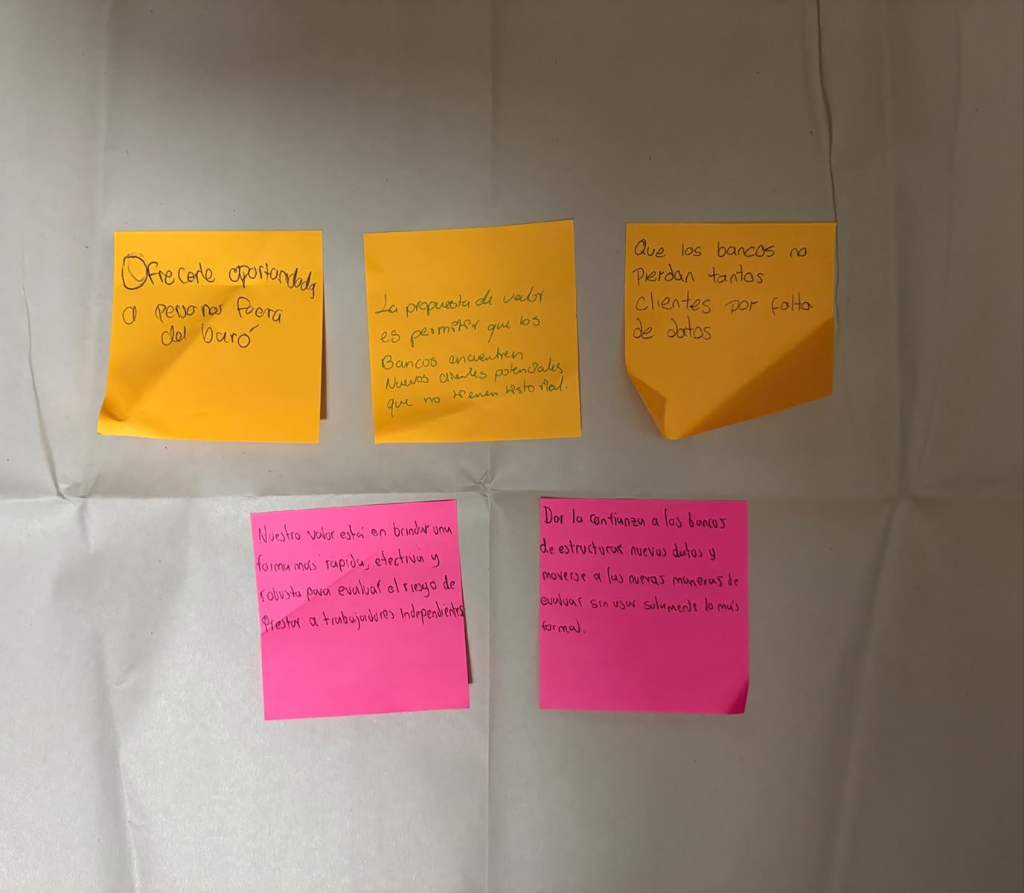
\includegraphics[width=0.75\textwidth]{trabajo_clase_2_octubre_2026.png}
    \caption{Evidencia de trabajo en clase: Taller creativo de definici\'on de propuesta y portafolio de valor (Sesi\'on del 2 de octubre de 2026).}
\end{figure}

\begin{tcolorbox}[colback=lightgray,colframe=primary,title={\textbf{S\'intesis de Post-its del Taller Creativo (2 de Octubre de 2026)}}]
\begin{itemize}[leftmargin=*]
    \item \textbf{Inclusi\'on y Acceso:} \textit{«Ofrecerle oportunidad a personas fuera del bur\'o».}
    \item \textbf{Crecimiento para la Entidad:} \textit{«La propuesta de valor es permitir que los bancos encuentren nuevos clientes potenciales que no tienen historial».}
    \item \textbf{Eficiencia y Datos:} \textit{«Que los bancos no pierdan tantos clientes por falta de datos».}
    \item \textbf{Velocidad y Precisi\'on:} \textit{«Nuestro valor est\'a en brindar una forma m\'as r\'apida, efectiva y robusta para evaluar el riesgo de prestar a trabajadores independientes».}
    \item \textbf{Confianza Regulatoria:} \textit{«Dar la confianza a los bancos de estructurar nuevos datos y moverse a las nuevas maneras de evaluar sin usar solamente lo m\'as formal».}
\end{itemize}
\end{tcolorbox}

\subsection{Primer Prototipo del Producto (MVP - Aulet Cap. 7)}
Dise\~no de alto nivel del flujo de funcionamiento del motor:

\begin{tcolorbox}[colback=lightgray,colframe=primary,title={\textbf{Flujo Operativo del Prototipo StatCredit AI}}]
\begin{enumerate}[leftmargin=*]
    \item \textbf{Paso 1 (Ingesta):} El solicitante autoriza y carga sus extractos digitales de Nequi o Daviplata en la aplicaci\'on de la entidad aliada.
    \item \textbf{Paso 2 (Procesamiento en API):} StatCredit AI ingesta el documento, ejecuta extracci\'on de transacciones y calcula m\'etricas de liquidez, frecuencia de clientes y persistencia de saldo.
    \item \textbf{Paso 3 (Modelo y Explicabilidad):} El modelo genera un puntaje entre 150 y 950 puntos, acompa\~nado de un reporte explicativo (m\'odulo SHAP) que detalla el impacto relativo de cada variable analizada.
    \item \textbf{Paso 4 (Entrega):} La entidad recibe en tiempo real el dictamen de aprobaci\'on, el cupo sugerido y el soporte t\'ecnico auditable para su archivo de riesgo SARC.
\end{enumerate}
\end{tcolorbox}

\newpage

% ---------------------------------------------------------
% SECCIÓN 4: CANALES Y RELACIÓN CON CLIENTES (AULET STEP 18)
% ---------------------------------------------------------
\section{Canales y Relaci\'on con Clientes (Sesi\'on 10 / Bloque 7)}

\subsection{Proceso de Adquisici\'on en Entidades Financieras (DMU)}
El proceso de venta B2B involucra a tres actores clave en la toma de decisi\'on:
\begin{itemize}[leftmargin=*]
    \item \textbf{Champion T\'ecnico (L\'ider de Producto / CTO):} Valora la facilidad de integraci\'on de la API, tiempos de latencia y estabilidad del servicio.
    \item \textbf{Oficial de Cumplimiento y Riesgo (SARC):} Requiere garant\'ia de que el modelo cumple con las directrices de la Superintendencia Financiera y no constituye una caja negra.
    \item \textbf{Comprador Econ\'omico (Gerencia / VP de Riesgo):} Analiza el balance entre el costo del software y el incremento en volumen de colocaci\'on con cartera sana.
\end{itemize}

\subsection{Embudo de Ventas a Corto, Mediano y Largo Plazo (Aulet Paso 18)}
Evoluci\'on comercial proyectada seg\'un el Paso 18 de Aulet:
\begin{enumerate}[leftmargin=*]
    \item \textbf{Corto Plazo (Meses 1 a 12 --- Entrada al Mercado):}
    \begin{itemize}
        \item \textit{Estrategia:} Venta directa (\textit{Field Sales}) mediante acercamiento personal de los fundadores con directores de riesgo de neobancos y fintechs aliadas.
        \item \textit{Herramienta de conversi\'on:} Pruebas piloto (PoC) de 30 d\'ias con extractos hist\'oricos para validar calibraci\'on del score frente a modelos existentes.
    \end{itemize}
    \item \textbf{Mediano Plazo (Meses 13 a 24 --- Tracci\'on):}
    \begin{itemize}
        \item \textit{Estrategia:} Venta consultiva interna (\textit{Inside Sales}) y participaci\'on activa en gremios como Colombia Fintech.
        \item Difusi\'on de casos de estudio que evidencien disminuci\'on en tiempos de evaluaci\'on y control de la mora.
    \end{itemize}
    \item \textbf{Largo Plazo (Meses 25 en adelante --- Escalamiento):}
    \begin{itemize}
        \item \textit{Estrategia:} Canal digital automatizado (\textit{Inbound / Internet Sales}) con documentaci\'on t\'ecnica abierta y portal de desarrolladores para integraci\'on inmediata.
    \end{itemize}
\end{enumerate}

\subsection{Relaci\'on con Clientes: Confianza, Soporte y Fidelizaci\'on B2B}
Como se establece en el Bloque 7 de la metodolog\'ia del curso (\textquestiondown C\'omo te conocen, te compran y regresan?), la relaci\'on con bancos peque\~nos y neobancos se basa en tres pilares de acompa\~namiento continuo:
\begin{itemize}[leftmargin=*]
    \item \textbf{Acompa\~namiento T\'ecnico Dedicado (Onboarding guiado):} En la fase de integraci\'on, nuestro equipo de ingenier\'ia brinda soporte directo a los desarrolladores de la entidad aliada, asegurando que la conexi\'on v\'ia API se realice en menos de dos semanas y sin fricciones operativas.
    \item \textbf{Garant\'ia de Servicio y Disponibilidad (SLA):} Aseguramos un acuerdo de nivel de servicio con disponibilidad del 99,9\% y tiempos de respuesta inferiores a 2 segundos por evaluaci\'on, protegiendo la experiencia del usuario en la aplicaci\'on m\'ovil del banco.
    \item \textbf{Soporte Regulatorio Permanente:} Ante cualquier actualizaci\'on normativa de la Superintendencia Financiera (circulares SARC), StatCredit AI recalibra los m\'odulos explicativos (SHAP) y genera la documentaci\'on t\'ecnica requerida, blindando jur\'idicamente a los comit\'es de riesgo aliados y consolidando una relaci\'on de largo plazo con tasa de deserci\'on (churn) proyectada inferior al 5\% anual.
\end{itemize}

\newpage

% ---------------------------------------------------------
% SECCIÓN 5: FUENTES DE INGRESO Y ECONOMÍA DEL NEGOCIO (AULET CAP. 15)
% ---------------------------------------------------------
\section{Fuentes de Ingreso y Econom\'ia del Negocio (Aulet Cap. 15)}

\subsection{Esquema de Cobro (Modelo SaaS B2B)}
Estructura de monetizaci\'on planeada para StatCredit AI:
\begin{enumerate}[leftmargin=*]
    \item \textbf{Tarifa Base Mensual de Plataforma:} Cuota fija de soporte, disponibilidad de infraestructura en la nube y mantenimiento continuo del motor anal\'itico (aproximadamente \$1.500 USD mensuales por entidad).
    \item \textbf{Cobro Variable por Consulta (\textit{Pay-per-Query}):} Tarifa escalonada por evaluaci\'on realizada:
    \begin{itemize}
        \item \$0,80 USD por consulta para paquetes iniciales (hasta 5.000 evaluaciones al mes).
        \item \$0,50 USD por consulta para vol\'umenes superiores a 10.000 evaluaciones mensuales.
    \end{itemize}
\end{enumerate}

\subsection{Viabilidad Financiera: Relaci\'on LTV vs. CAC}
\begin{itemize}[leftmargin=*]
    \item \textbf{Costo de Adquisici\'on de Clientes (CAC estimado):} Calculado en aproximadamente \$4.000 USD por entidad vinculada, considerando ciclo de venta comercial, horas de ingenier\'ia en pilotos y validaci\'on jur\'idica.
    \item \textbf{Valor de Vida del Cliente (LTV proyectado):} Debido al alto costo de sustituci\'on de infraestructura de riesgo en entidades financieras, se proyecta una permanencia m\'inima de 36 meses con ingresos promedio de \$60.000 USD por cliente institucional.
    \item \textbf{Relaci\'on LTV / CAC:} La raz\'on resultante supera \textbf{15 veces} el CAC, cumpliendo con holgura el criterio metodol\'ogico de Aulet ($\text{LTV} \ge 3\times \text{CAC}$), con recuperaci\'on de la inversi\'on comercial en los primeros meses de operaci\'on.
\end{itemize}

\newpage

% ---------------------------------------------------------
% SECCIÓN 6: PRIMER LIENZO DE MODELO DE NEGOCIO (ZONA ENTREGAR: P1 - P3)
% ---------------------------------------------------------
\section{Primer Lienzo de Portafolio de Valor (Zona Entregar: P1 -- P3)}

\begin{tcolorbox}[colback=primary!5,colframe=primary,title={\textbf{Estructura Metodol\'ogica del Primer Lienzo}}]
De acuerdo con las indicaciones de la Sesi\'on 10, el modelo de negocio se construye de forma progresiva. En este entregable consolidamos el \textbf{Primer Lienzo Canvas}, centrado en la \textbf{Zona ENTREGAR (P1 a P3)}: conectando el Problema validado (Bloque 1 / P1), los Segmentos de Actores (Bloque 2 / P1), el Portafolio de Valor (Bloque 3 / P2) y los Canales junto con la Relaci\'on con Clientes (Bloque 7 / P3). Los bloques de Capturar (Costos e Ingresos / P4) y Compartir (Impacto y ODS / P6) se formalizar\'an en las fases siguientes del proyecto.
\end{tcolorbox}

\vspace{0.4cm}

\begin{table}[htbp]
\centering
\small
\begin{tabularx}{\textwidth}{|X|X|}
\hline
\rowcolor{primary!10}
\multicolumn{2}{|c|}{\textbf{\Large ZONA ENTREGAR VALOR (Portafolios 1 al 3)}} \\
\hline
\textbf{Bloque 1 (P1): Problema y Oportunidad} \newline
\textit{\textquestiondown Qu\'e dolor real vale la pena resolver?} & 
\textbf{Bloque 2 (P1): Segmentos de Actores} \newline
\textit{\textquestiondown A qui\'en sirves y a qui\'en afectas?} \\
\hline
$\bullet$ Asimetr\'ia de informaci\'on: Bancos rechazan al 65\% de independientes solventes por falta de n\'omina fija. \newline
$\bullet$ Cuello de botella operacional: Revisi\'on manual de extractos limita a 15--20 casos al d\'ia por analista. \newline
$\bullet$ Exclusi\'on financiera empuja a micronegocios al cr\'edito usurero (``gota a gota'' al 20\%--40\% mensual). \newline
$\bullet$ Temor a sanciones SARC por modelos opacos de ``caja negra''. & 
$\bullet$ \textbf{Cliente que paga (B2B):} Neobancos, bancos peque\~nos y cooperativas financieras en Colombia que buscan crecer su cartera. \newline
$\bullet$ \textbf{Beneficiario final (B2B2C):} 4,5 millones de trabajadores independientes y comerciantes urbanos con actividad digital (Nequi/Daviplata/DIAN). \newline
$\bullet$ \textbf{Otros actores:} Analistas de cr\'edito, comit\'es de riesgo, gremios fintech y la Superintendencia Financiera. \\
\hline
\textbf{Bloque 3 (P2): Portafolio de Valor} \newline
\textit{\textquestiondown Qu\'e valor multidimensional creas?} & 
\textbf{Bloque 7 (P3): Canales y Relaci\'on con el Cliente} \newline
\textit{\textquestiondown C\'omo te conocen, te compran y regresan?} \\
\hline
$\bullet$ \textbf{Core Business (Usuario):} Evaluaci\'on justa en $<2$ segundos con explicaci\'on transparente de factores de solvencia. \newline
$\bullet$ \textbf{Econ\'omica (Profit):} Incremento del 20\% al 30\% en originaci\'on sana de cr\'edito para bancos peque\~nos. \newline
$\bullet$ \textbf{Social (People):} Alternativa formal y digna frente a la usura informal. \newline
$\bullet$ \textbf{Ambiental (Planet):} Cero papel; proceso 100\% en la nube y energ\'ia eficiente. & 
$\bullet$ \textbf{Canales de Adquisici\'on:} Venta directa (\textit{Field Sales}) a comit\'es de riesgo, pruebas piloto (PoC) de 30 d\'ias y eventos en Colombia Fintech. \newline
$\bullet$ \textbf{Canal de Entrega:} REST API segura con integraci\'on r\'apida en $<2$ semanas. \newline
$\bullet$ \textbf{Relaci\'on y Confianza:} Onboarding guiado, soporte t\'ecnico 24/7 con SLA del 99,9\% y actualizaci\'on regulatoria continua bajo norma SARC. \\
\hline
\end{tabularx}
\caption{Primer Esquema del Lienzo Canvas --- Consolidado de la Zona Entregar (P1 a P3).}
\end{table}

\end{document}